\documentclass[tikz,border=10pt]{standalone}
\usepackage{amsmath}
\usepackage{amssymb}
\usetikzlibrary{shapes,arrows,positioning,fit,matrix,decorations.pathreplacing}

\begin{document}
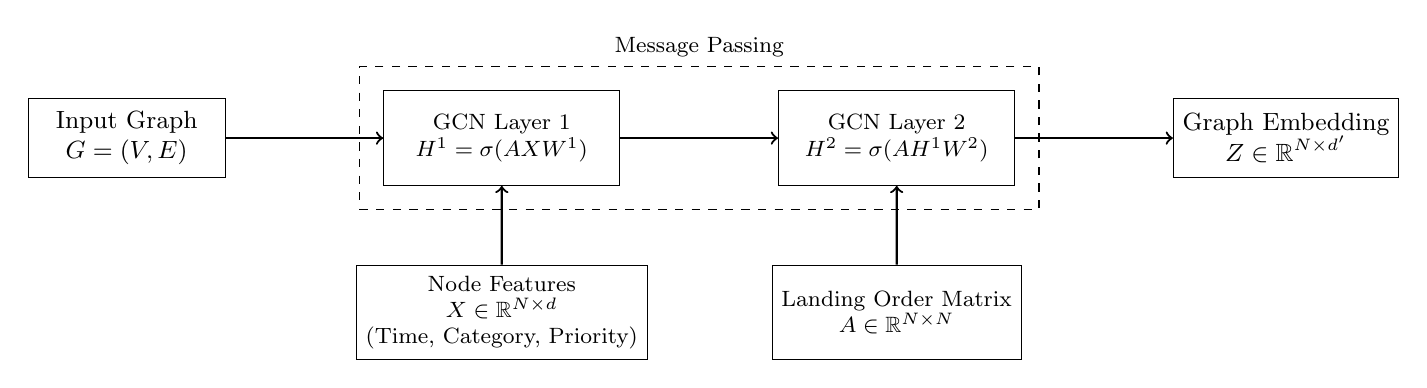
\begin{tikzpicture}[
    scale=0.8,
    node distance=2cm,
    box/.style={
        rectangle,
        draw,
        minimum width=2.5cm,
        minimum height=1cm,
        font=\small,
        align=center
    },
    layer/.style={
        rectangle,
        draw,
        minimum width=3cm,
        minimum height=1.2cm,
        font=\footnotesize,
        align=center  % Crucial fix for line breaks
    },
    arrow/.style={->,thick}
]

% Input Graph
\node[box] (input) {Input Graph\\$G=(V,E)$};

% Graph Convolution Layers
\node[layer, right=2cm of input] (gcn1) {
    GCN Layer 1\\
    $H^1 = \sigma(AXW^1)$
};
\node[layer, right=2cm of gcn1] (gcn2) {
    GCN Layer 2\\
    $H^2 = \sigma(AH^1W^2)$
};

% Node Feature Processing
\node[layer, below=1cm of gcn1] (feat) {
    Node Features\\
    $X \in \mathbb{R}^{N \times d}$\\
    (Time, Category, Priority)
};
\node[layer, below=1cm of gcn2] (adj) {
    Landing Order Matrix\\
    $A \in \mathbb{R}^{N \times N}$
};

% Output
\node[box, right=2cm of gcn2] (output) {Graph Embedding\\$Z \in \mathbb{R}^{N \times d'}$};

% Connections
\draw[arrow] (input) -- (gcn1);
\draw[arrow] (gcn1) -- (gcn2);
\draw[arrow] (gcn2) -- (output);
\draw[arrow] (feat) -- (gcn1);
\draw[arrow] (adj) -- (gcn2);

% Message Passing Illustration (corrected)
\node[rectangle,draw,dashed,fit=(gcn1)(gcn2),  % No space between nodes
      inner sep=0.3cm,
      label={[above,font=\footnotesize]Message Passing}] {};

\end{tikzpicture}
\end{document}
